\chapter{具有完美信息的博弈树}
\label{chp: 具有完美信息的博弈树}

本章讨论博弈树，它是除策略型之外定义非合作博弈的另一种主要方式。在博弈树中，参与人依次行动，并且在本章所研究的完美信息情形下，每个参与人都知道其他参与人此前的行动。相比之下，参与人在策略型博弈中是同时行动的。在这种“动态”的环境下，一次博弈进程是指由参与人的一系列行动所确定的一次具体博弈过程。

博弈树由一棵树来表示，其节点代表可能的博弈状态。一些节点是机会节点，在这些节点上，下一个节点根据已知的概率分布随机确定。决策节点则属于某个参与人，由该参与人选择行动，从而确定下一个节点。博弈在博弈树的终端节点或叶节点处结束，此时每个参与人获得相应的收益。

博弈树可以通过逆向归纳法求解。其基本思想是，在假定所有后续行动均已确定的情况下，为每个参与人寻找最优行动。逆向归纳法从最接近叶节点的决策节点开始，并假定参与人总是选择使其收益最大化的行动。一般而言，这样的最优行动未必唯一，因此，通过逆向归纳法确定的不同参与人的行动可能彼此依赖(见图\ref{fig:4.4})。

博弈树中的策略是一个由行动衍生出来的概念。一个策略规定了参与人在自己的每个决策节点上应采取的行动，因此构成了针对每一种可能博弈状态的完整行动计划。于是，任意一个策略组合都会确定每个参与人的收益(如果博弈中存在机会行动，则可能是期望收益)，由此便可以得到该博弈的策略式。

由于每个策略都是多个行动的组合，博弈树中的策略数量往往非常庞大。精简策略可以在一定程度上减少策略的数量。在一个精简策略中，如果某个决策节点由于参与人自己先前采取的行动而不可能到达，那么无需规定该参与人在这一节点上的行动。

逆向归纳法确定的策略组合构成该博弈的一个均衡(定理~\ref{theo:4.6})。这一均衡称为子博弈精炼纳什均衡（SPE），因为它在每个子博弈中都构成均衡。(在完美信息博弈树中，一个子博弈就是原博弈树的一棵子树。而在第10章讨论的不完美信息博弈中，一般而言，不能通过逆向归纳法求得子博弈精炼纳什均衡。)

在第 4.7 节中，我们将讨论承诺博弈。这是一类两人博弈，将策略型博弈改写为博弈树：其中一个参与人先行动，另一个参与人知晓第一个参与人的行动并对此做出反应。假设后行动的参与人总是选择最优反应，就像在子博弈精炼纳什均衡中一样。这样的行动顺序改变了原有博弈，而且通常有利于先行动者。我们将研究质量博弈以及第3.6节数量竞争的古诺双寡头博弈所对应的承诺博弈。在后一种情形中，这种承诺博弈称为斯塔克尔伯格领导者博弈。

每个博弈树都可以转换为策略型博弈。反过来，一个一般的策略型博弈只有在博弈树中加入用于描述不完美信息的额外结构后，才能表示为博弈树。不完美信息博弈树将在第10章讨论。

\section{预备知识和学习目标}

第 3 章是学习本章的预备知识，第 1 章则不是。尽管如此，第1章中的组合博弈也是本章所研究的完美信息序贯博弈，因此可以作为有助于理解本章内容的例子。作为背景知识，我们还将回顾有向图、树以及随机变量期望值等数学概念。

学习本章后，你应该能够
\begin{itemize}
\item 解读博弈树及其行动和收益；
\item 把参与人的行动组合成策略，并掌握如何计算策略数量；
\item 将策略归并为精简策略，识别由于参与人自己先前的行动而无法到达的决策节点上的行动，并理解表示策略的行动列表中相应的“*”通配符应放在何处；
\item 写出博弈树对应的策略型，将参与人的收益正确地放置在每个单元格中，并在需要时计算期望收益；
\item 解释逆向归纳法以及为什么它需要完整(未精简)的策略，以及由此得到的策略为什么可能不是唯一的；
\item 直接从博弈树构建均衡，即使该均衡不是子博弈精炼纳什均衡。这一方法也适用于两个以上参与人的情形，如练习~\ref{exer:4.5} 所示；
\item 从策略型博弈中构建承诺博弈，并将比较其子博弈精炼纳什均衡与策略形式中的均衡。
\end{itemize}

\section{博弈树的定义}

图\ref{fig:4.1}展示了一个博弈树的例子。我们总是将树从上向下绘制，并将起始节点(称为根节点)置于最上方。(博弈树的绘制方法并不统一：有时树从下向上绘制，有时从左向右绘制，有时将根节点置于中心，边可以向任意方向延伸。)

  \begin{figure}[H]
    \centering
    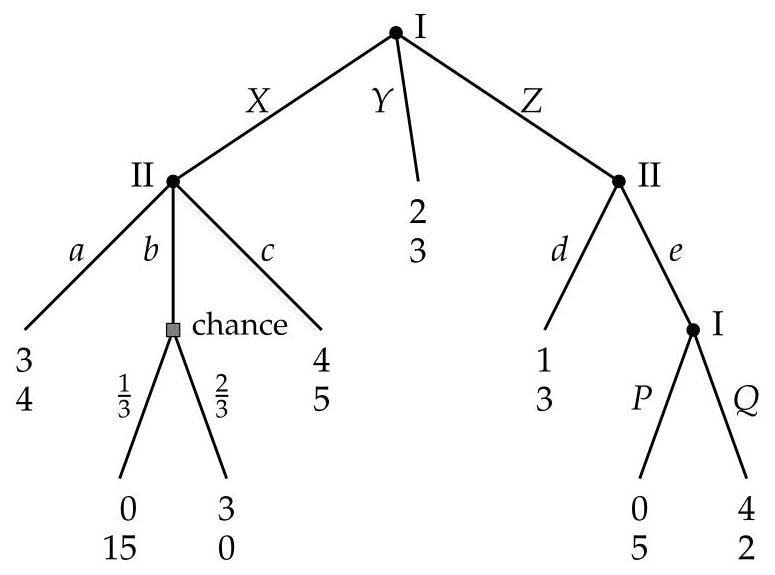
\includegraphics[width=0.6\linewidth]{translation/images/ch04-fig01.jpg}
    \caption{博弈树示例。方形节点表示机会节点。在博弈树的叶节点处，上方的收益属于参与人 I，下方的收益属于参与人 II。}
    \label{fig:4.1}
  \end{figure}

图\ref{fig:4.1}中树的节点表示博弈状态(在第 1 章讨论的组合博弈中被称为“位置”)。节点之间由线相连，这些线称为边。从节点 \(u\) 到其子节点 \(v\) (其中 \(v\) 绘制在 \(u\) 下方)的一条边表示博弈中的一个可能行动。这一行动可以由某个参与人作出，例如图\ref{fig:4.1}中参与人 I 的行动 \(X\) ，此时 \(u\) 也称为决策节点。 \(u\) 也可能是一个机会节点，如图\ref{fig:4.1}中参与人 II 行动 \(b\) 之后的节点 \(u\) 。我们将决策节点绘制为小实心圆，将机会节点绘制为方形。在机会节点 \(u\) 之后，下一个节点 \(v\) 由与从 \(u\) 到 \(v\) 的边相关联的概率随机确定。在图\ref{fig:4.1}中的机会节点上，向左行动的概率为 \(\frac{1}{3}\) ，向右行动的概率为 \(\frac{2}{3}\) 。

在博弈树的终端节点或叶节点处，每个参与人都会获得相应的收益。在图\ref{fig:4.1}中，叶节点未明确绘制，而是直接标出了收益，上方的收益属于参与人 I，下方的收益属于参与人 II。

树的绘制方式并不重要，重要的是节点如何通过边连接，相关概念已在下面关于有向图和树的背景材料中作了介绍。下面给出博弈树的正式定义。

\begin{mybox}{背景材料：有向图与树}
\setlength{\parindent}{2em}

有向图（directed graph，也称 digraph）由有限的节点集合和有限的边集合构成。每条边都是两个节点 \(u\) 和 \(v\) 构成的有序对，记作 \(uv\)。从 \(u\) 到 \(v\) 的一个游走（walk）是一个节点序列 \(u_0,u_1,\ldots,u_m\)，其中 \(m\geq 0\)，对于 \(0\leq k<m\)，\(u_ku_{k+1}\) 都是一条边，并且 \(u=u_0\)、\(v=u_m\)。如果这些节点彼此不同，则这一游走称为一条路径（path）。

一棵（有向）树是一个具有指定节点的有向图，这一指定节点称为根节点（root），并且对于每个节点 \(u\)，从根节点到 \(u\) 都存在唯一的游走。如果 \(uv\) 是树中的一条边，则 \(v\) 称为 \(u\) 的子节点（child），\(u\) 称为 \(v\) 的父节点（parent）。在一棵树中，如果从节点 \(u\) 到节点 \(v\) 存在非空游走，则称 \(v\) 是 \(u\) 的后代节点（descendant）。没有子节点的节点称为树的叶节点（leaf）或终端节点（terminal node）。

我们通常将树画成根节点位于顶部，并将边从父节点向下画至子节点。

\begin{lemma}\label{lem:4.1}
在一棵树中，从根节点到任一节点的唯一游走都是一条路径。除根节点没有父节点外，每个节点都有唯一的父节点。
\end{lemma} 
\begin{proof}
如果从根节点 \(u_0\) 到节点 \(u_m\) 的游走 \(u_0,u_1,\ldots,u_m\) 中存在重复节点，即对于某个 \(i<j\)，有 \(u_i=u_j\)，那么我们可以从该游走中删去节点 \(u_{i+1},\ldots,u_j\)，从而得到另一条从 \(u_0\) 到 \(u_m\) 的游走，这与从根节点到每个节点的游走具有唯一性相矛盾。因此，该游走中不存在重复节点，所以它是一条路径。

考虑一个不是根节点的节点 \(u\)，设 \(vu\) 是从根节点到 \(u\) 的唯一路径上的最后一条边。如果还存在另一条边 \(wu\)，其中 \(w\neq v\)，那么从根节点到 \(w\) 的路径再接上边 \(wu\)，就会得到另一条从根节点到 \(u\) 的路径，这与唯一性相矛盾。因此，\(v\) 是 \(u\) 的唯一父节点。如果根节点存在一个父节点 \(v\)，那么从根节点到 \(v\) 的路径再接上从 \(v\) 到根节点的边，就会形成一条从根节点到自身的非空游走；另一方面，还存在仅由根节点自身构成的长度为 \(0\) 的游走。这样，从根节点到自身就存在两条不同的游走，这同样与唯一性相矛盾。    
\end{proof} 
\end{mybox}


\begin{definition}\label{def:4.2}
博弈树是具有以下信息的树：

\begin{itemize}
\item 有限个参与人，共 \(N\) 人。
\item 树的每个非终端节点要么是属于某个参与人的决策节点，要么是机会节点。
\item 对于一个决策节点 \(u\) ，从该节点到其子节点 \(v\) 的每条边 \({uv}\) 都代表了一个不同的行动。这些行动被称为在节点 \(u\) 处的行动。
\item 对于一个机会节点 \(u\) ，从该节点到其子节点 \(v\) 的边 \({uv}\) 被赋予概率(即非负实数且其和为 1)。
\item 博弈树的每个叶节点都有一个 \(N\) 元实值收益向量，每个参与人对应一个收益值。
\end{itemize}
\end{definition}

参与人知道整个博弈树，包括其中的决策节点、行动、机会概率和收益，这些信息完整地定义了该博弈。博弈从根节点开始进行。在决策节点处，相应的参与人选择一个行动，该行动决定下一个节点。在机会节点处，按照给定概率随机选择行动。当到达叶节点时，博弈结束，所有参与人获得相应收益。参与人目标是最大化自己的收益。如果博弈结果具有随机性，则假设参与人的目标是最大化自己的期望收益。


\begin{mybox}{背景材料：有限随机变量的期望值}
\setlength{\parindent}{2em}

随机变量 \(U\) 取实数值，其取值取决于随机事件的结果。设 \(U\) 取有限个值 \(u_1,\ldots,u_k\)，这些值分别以概率 \(p_1,\ldots,p_k\) 出现。那么，\(U\) 的期望值或期望定义为
\begin{equation}\label{eq:4.1}
\mathbb{E}[U] = p_1u_1+\cdots+p_ku_k.
\end{equation}
由于概率 \(p_1,\ldots,p_k\) 之和为 \(1\)，因此期望值就是以相应概率 \(p_i\) 为权重，对各个取值 \(u_i\) 计算得到的加权平均值。

作为一种特殊情况，如果随机变量是确定性的，并且仅取一个值 \(u_1\)（其概率为 \(p_1=1\)），那么该值本身就是其期望值，即 \(\mathbb{E}[U]=u_1\)。

\end{mybox}

在图\ref{fig:4.1}中，机会行动之后参与人 I 的期望收益是 \(\frac{1}{3}\times0 + \frac{2}{3}\times3 = 2\)，参与人 II 的期望收益是 \(\frac{1}{3}\times{15} + \frac{2}{3}\times0 = 5\)。因此，在这个博弈中，可以将这一机会节点替换为一个叶节点，并令参与人 I 和参与人 II 在该叶节点处的收益分别为 2 和 5。这些期望收益反映了参与人对于随机结果的偏好；第 5 章将详细讨论采用这种收益表示所依据的假设。在两人博弈中，我们通常将参与人命名为参与人 I 和参与人 II。参与人 I 的行动通常用大写字母表示，参与人 II 的行动通常用小写字母表示。

图\ref{fig:4.2}说明了树的一个基本性质：从根节点到每个节点都存在唯一的路径。左图\ref{fig:4.2}(a)中的中间叶节点并不满足这一性质。不过，这样的结构在描述某些博弈时看起来可能是合理的。例如，该图可以表示酒吧里的两个人：在第一轮中，参与人 I 首先决定是自己为酒水买单（行动 \(P\)），还是接受由参与人 II 买单（行动 \(A\)）。在第二轮中，参与人 II 再决定是不买单（行动 \(a\)），还是买单（行动 \(p\)）。参与人可能只关心自己总共买了几轮单，而不关心具体在哪一轮买单。这样，中间的收益对 \((1,1)\) 就可能对应两种不同的行动“历史”。树的性质排除了一个博弈状态具有多个历史的情形，因为一个状态的历史由从根节点到该状态的唯一路径表示。即使博弈历史中的某些差异并不重要，我们仍然将这些博弈状态区分开来，这主要是出于数学处理上的便利。上述博弈的正确表示如右图\ref{fig:4.2}(b)所示。

\begin{figure}[H]
\centering
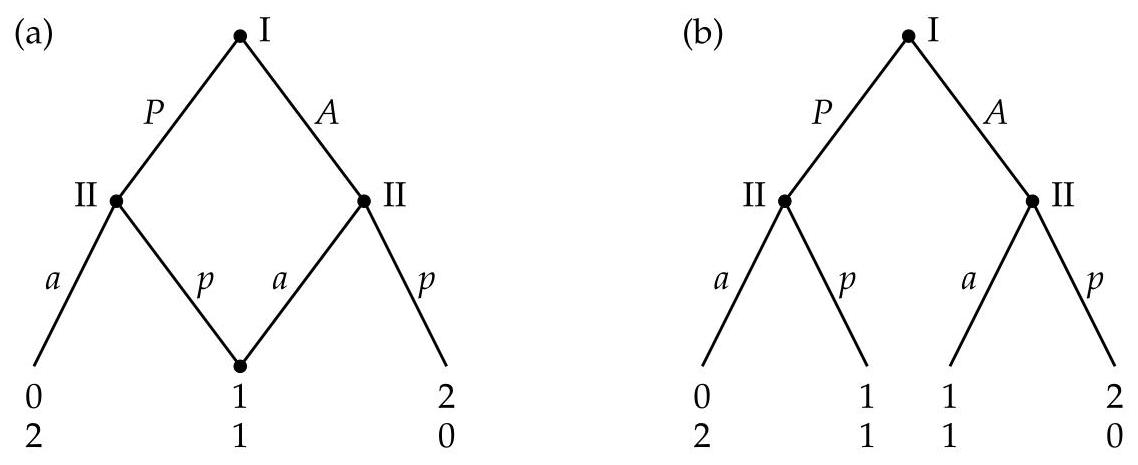
\includegraphics[width=0.8\linewidth]{translation/images/ch04-fig02.jpg}
\caption{左图(a)不是一棵博弈树，因为两个参与人收益都为1的叶节点可以通过两条不同的路径到达。正确的博弈树表示如右图(b)所示。}
\label{fig:4.2}
\end{figure}

由博弈树表示的博弈也称为完美信息扩展式博弈。完美信息是指参与人在行动时总是知道当前的博弈状态，因而也知道此前完整的博弈历史。通过在博弈树中加入额外的结构，还可以表示不完美信息，这是第10章讨论的主题。表示同时行动需要引入不完美信息。在本章所考虑的博弈树中，参与人依次行动，并且能够观察到其他参与人的行动。

注意博弈树与第 1 章中的组合博弈有以下区别：
\begin{itemize}
\item 组合博弈可以非常简洁地描述，尤其是在将其表示为若干博弈之和时。对于一般的博弈树，通常不考虑这样的博弈之和。
\item 博弈树中的规则更加灵活：允许有两个以上的参与人，也可以包含机会行动，参与人不必交替行动，收益也不仅代表“赢”或“输”。
\item 然而，博弈树的灵活性是有代价的：博弈的描述比组合博弈长得多。例如，一个简单的尼姆博弈可能需要一个巨大的博弈树。像mex规则这样的规律并不适用于一般的博弈树。
\end{itemize}

\section{逆向归纳法}

在博弈树中，参与人应该选择哪些行动？最优行动应该使参与人自己的收益最大化。如果某个参与人是最后行动者，那么他的最优行动可以不考虑其他参与人的行动而直接确定。在图\ref{fig:4.3}(a)的博弈中，参与人 II 选择行动 \(r\) 可以使自己的收益最大化。从后向前考虑，参与人 I 在博弈树的根节点选择 \(T\) 或 \(B\)。假定参与人 II 随后采取上述行动，参与人 I 选择这两个行动所获得的收益分别为 1 和 2。因此，他会选择 \(B\)，最终两个参与人的收益均为 2。这些选定的行动在图\ref{fig:4.3}(b)中用边上的箭头表示。与我们在策略型博弈中用方框标出最优反应对应的收益类似，这些箭头只是为了帮助分析博弈而添加的信息，并不属于博弈本身的定义。

  \begin{figure}[H]
    \centering
    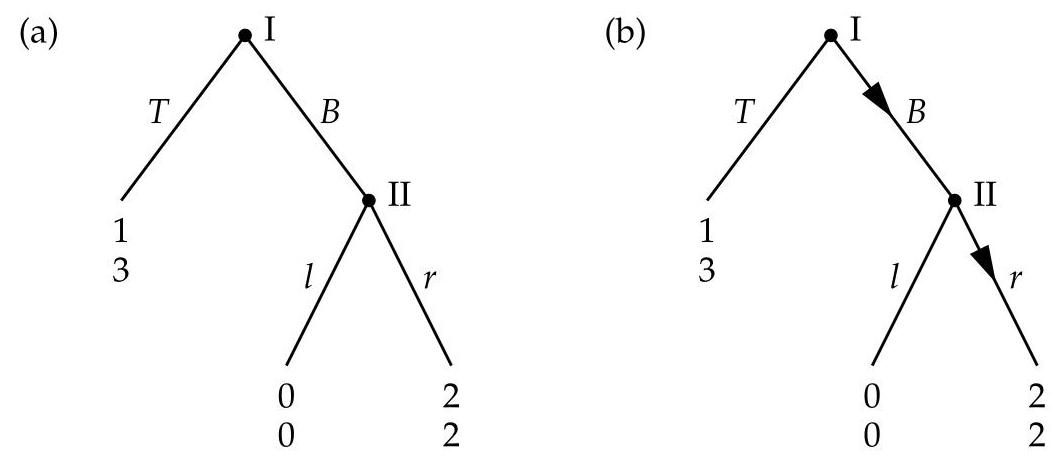
\includegraphics[width=0.8\linewidth]{translation/images/ch04-fig03.jpg}
    \caption{一个两人博弈树(a)以及通过逆向归纳法选出的行动(b)。}
    \label{fig:4.3}
  \end{figure}


这一过程称为逆向归纳法：从最接近叶节点的决策节点开始，在每个决策节点处，选择一个使该节点所属参与人的收益最大化的行动。一般而言，只要某个决策节点之后的所有行动都已经确定，就可以用这种方式确定该节点处的行动。最终，每个决策节点处的行动都会被确定，从而得到整个博弈的一套行动选择。

  \begin{figure}[H]
    \centering
    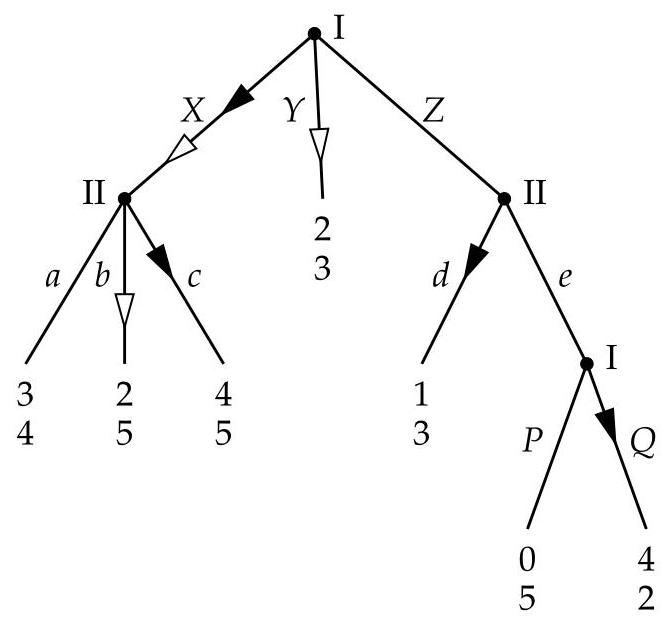
\includegraphics[width=0.6\linewidth]{translation/images/ch04-fig04.jpg}
    \caption{图\ref{fig:4.1}中的博弈树，机会行动被其期望收益所取代，逆向归纳法所确定的行动取决于参与人 II 在 \(b\) 和 \(c\) 之间的选择：若选择 \(b\)（白色箭头），参与人 I 随后可以选择 \(X\) 或 \(Y\)；若选择 \(c\)（黑色箭头），参与人 I 唯一的选择是 \(X\)。}
    \label{fig:4.4}
  \end{figure}


如果有不止一种行动能为参与人带来最大收益，那么逆向归纳法所选择的行动不一定是唯一的，这还可能影响博弈树中更早节点处的行动选择。在图\ref{fig:4.4}的博弈中，逆向归纳法为参与人 II 选择行动 \(b\) 或行动 \(c\) ，这两种行动都能为她带来收益 $5$（这是图\ref{fig:4.1}原始博弈中行动 \(b\) 的期望收益)，超过了她选择行动 \(a\) 时的收益 $4$。在最右侧的节点，参与人 I 选择 \(Q\) 。这决定了参与人 II 的前一个行动 \(d\) ，该行动为她带来了更高的收益 $3$，而不是 $2$（通过行动 \(Q\) )。反过来，这意味着参与人 I 在博弈树的根节点选择 \(X,Y\) 或 \(Z\) 时，选择 \(Y\) 能得到收益 $2$，选择 \(Z\) 能得到收益 $1$。他选择 \(X\) 时的收益取决于参与人 II 的选择：如果参与人 II 选择 \(b\) ，那么参与人 I 得到 2，他可以选择 \(X\) 或 \(Y\) ，这两种选择都能为他带来最大收益 $2$。这些选择在图\ref{fig:4.4}中用白色箭头表示。然而，如果参与人 II 选择 \(c\) ，那么参与人 I 选择 \(X\) 时的收益是 $4$，所以 \(X\) 是唯一的最优行动。

综上所述，通过逆向归纳法在图\ref{fig:4.1}中可能出现的行动组合，按每个参与人的行动列出为: \(\left( {{XQ},{bd}}\right) ,\left( {{XQ},{cd}}\right)\) 和 \((YQ,bd)\)。请注意， \(Q\) 和 \(d\) 总是会被选择，但 \(Y\) 只能与参与人 II 的行动 \(b\) 组合选择。

我们并不试图主张，参与人 II 因为存在参与人 I 可能选择 \(Y\) 的“风险”，就“不应该”选择 \(b\)。这样的论证相当于对逆向归纳法作进一步的“精炼”，这里不讨论这种做法。

因此，一般来说，逆向归纳法所确定的行动并非唯一，而且不同节点处的行动选择还可能相互依赖。

如果在每个决策节点处总是只有一个行动能够带来最大收益，那么逆向归纳法就会为每个参与人给出唯一的行动建议。这种情况适用于一般博弈（generic games）。所谓一般博弈，是指其收益参数为实数，并且这些参数之间不存在特殊的依赖关系，例如两个收益恰好相等。特别地，对这些收益参数作小幅扰动应当不会产生问题。例如，在某些实际情形中，收益可能受到某种“噪声”的影响，从而使每个收益的精确数值发生轻微变化。在这种情况下，两个收益恰好相等的概率为零，因此可以忽略这种情形。在一般博弈中，每个决策节点处的最优行动都是唯一的，因此逆向归纳法会给出唯一的结果。

\section{博弈树中的策略}

在策略型博弈中，每个参与人的策略被视为给定的。对于扩展式博弈，策略是一个派生概念。理解博弈树中策略的最好方式，是将其看作针对参与人每个决策节点所制定的行动计划。

\begin{definition}\label{def:4.3}
    在博弈树中，参与人的策略为该参与人的每个决策节点指定一个行动。
\end{definition} 

因此，如果一个参与人有 \(k\) 个决策节点，那么该参与人的策略就是一个由 \(k\) 个行动组成的元组。为了符号表示的简便，我们通常将策略写成一个行动列表，每个行动对应参与人的一个决策节点(而不是用括号括起来、用逗号分隔的元组)。在图\ref{fig:4.1}的博弈树中，参与人 I 的策略是 \({XP},{XQ},{YP},{YQ},{ZP},{ZQ}\) 。参与人 II 的策略是 \({ad},{ae},{bd}, {be}, {cd},{ce}\) 。以这种方式指定策略时，必须按照树中决策节点的固定顺序进行，以便唯一地识别每个行动。当一个行动名称出现多次时，这一点很重要，例如在图\ref{fig:4.2}(b)中。在该树中，参与人 II 的策略是 \({aa},{ap},{pa},{pp}\) ，要理解为第一个行动对应参与人 II 的左决策节点，第二个行动对应右决策节点。

逆向归纳法为博弈树的每个决策节点定义一个行动，因此也为每个参与人的每个决策节点定义一个行动，进而为每个参与人确定了一个策略。因此，逆向归纳法的结果是一个策略组合。

有了每个参与人的策略，我们就可以定义该博弈树所对应的策略形式，具体如下。考虑一个策略组合，并假设所有参与人都按照各自的策略行动。如果不存在机会行动，那么这些策略将唯一确定一个叶节点。如果存在机会行动，那么一个策略组合可能在博弈树的各个叶节点上诱导出一个概率分布，并由此产生期望收益。当机会行动出现在博弈树较靠前的位置时，期望收益的计算会比图\ref{fig:4.1}中的情形更为复杂；图\ref{fig:4.8}给出了一个例子。一般而言，任何一个策略组合都会为每个参与人确定一个期望收益；其中也包括确定性的情形，此时收益与期望收益相同，正如式\ref{eq:4.1}之后所述。

\begin{definition}
    扩展式博弈的策略形式由根据定义\ref{def:4.3}为每个参与人设定的策略集以及每个策略组合为每个参与人带来的期望收益来定义。
\end{definition}

我们首先考虑图\ref{fig:4.3}中的简单博弈树，它与它的策略形式(已经在图\ref{fig:3.6}中见过)一起显示在图\ref{fig:4.5}中，这是一个 \(2 \times  2\) 博弈。在这个博弈中，每个参与人只有一个决策节点，因此策略与行动相同。(一般来说，策略指定多个行动，因此不要将“策略”和“行动”这两个术语互换使用！)还要注意，我们在博弈树的每个叶节点的顶部写出参与人 I 的收益，但在收益表中一个单元格的左下角写出。

图\ref{fig:4.3}中的博弈树只有三个叶节点(且没有机会行动)，但策略形式有四个单元格。因此，其中一个叶节点的收益会出现两次，即对应于策略对 $(T,l)$和$(T,r)$。原因是，在参与人 \(\mathrm{I}\) 采取行动 \(T\) 后立即到达最左边的叶节点，然后参与人 II 的行动 \(l\) 或 \(r\) 就无关紧要了。

  \begin{figure}[H]
    \centering
    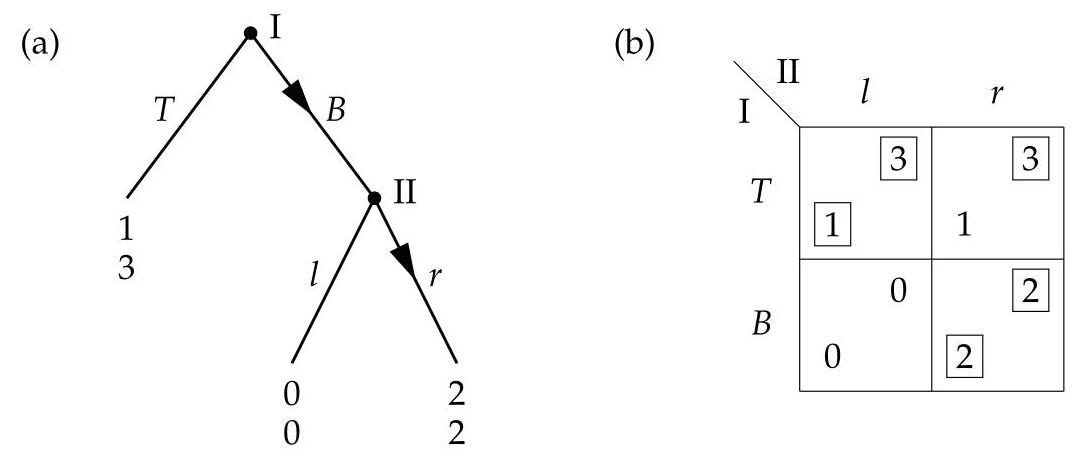
\includegraphics[width=0.8\linewidth]{translation/images/ch04-fig05.jpg}
    \caption{带有逆向归纳法步骤的威胁博弈博弈树(a)及其带有最优反应的策略形式(b)。注意：在博弈树中，参与人 I 的收益显示在顶部，但在策略形式中，它们出现在每个单元格的左下角。}
    \label{fig:4.5}
  \end{figure} 

博弈树和策略形式描述的是同一个博弈，但玩法不同。在博弈树中，博弈按顺序进行。在策略形式中，参与人同时选择他们的策略，然后根据这些行动计划进行博弈。

在图\ref{fig:4.5}的博弈中，逆向归纳法确定了唯一的策略组合 $(B,r)$，这也是一个均衡(一般情况下都成立，见下面的定理~\ref{theo:4.6})。该博弈还存在另一个均衡 \((T,l)\)，这一点也可以从博弈树中看出：如果参与人 II 选择 \(l\)，那么参与人 I 的最优反应就是 \(T\)。参与人 II 可以以这一并非最优的行动相威胁，因为一旦参与人 I 选择 \(T\)，参与人 II 的决策节点便不会被到达，因此她实际上永远不需要采取 \(l\)；而这一威胁又会使参与人 I 有动机选择 \(T\)。正因如此，这个博弈也被称为威胁博弈。在均衡 \((T,l)\) 中，参与人 II 获得的收益更高。我们将在第~\ref{sec:4.6} 节区分通过逆向归纳法得到的均衡与不能通过逆向归纳法得到的均衡。

图\ref{fig:4.6}给出了图\ref{fig:4.1}中博弈树的策略形式。在该博弈中，参与人 I 和参与人 II 都各有两个决策节点，并且在各自的两个决策节点处分别有三个和两个可选行动，因此每个参与人都有 \(3\times2\) 个策略，策略形式有$36$个单元格，由于博弈树本身只有八个叶节点（或者像图\ref{fig:4.4}那样，将机会节点的两个随机结果合并后只有七个叶节点），这些单元格中会出现许多重复的收益。

\section{精简策略}

在图\ref{fig:4.6}中，两行 \({XP}\) 和 \({XQ}\) 对两个参与人来说收益相同，同样，两行 \({YP}\) 和 \({YQ}\) 也是如此。原因是策略 \({XP}\) 和 \({XQ}\) 规定参与人 I 在他的第一个决策节点选择 \(X\) ，在他的第二个决策节点选择 \(P\) 或 \(Q\) 。然而，在选择 \(X\) 之后，无法到达第二个决策节点。只有当参与人 I 将 \(Z\) 作为他的第一步行动时，才能到达第二个决策节点，然后两种策略 \({ZP}\) 和 \({ZQ}\) 可能会导致不同的叶节点(如果参与人 II 选择 \(e\) ，就像她的三种策略 \({ae},{be}\) 或 \({ce}\) 那样)。因为参与人 I 自己在 \(X,Y\) 或 \(Z\) 之间进行选择，所以用一个不太具体的“行动计划” \(X *\) 来取代策略 \({XP}\) 和 \({XQ}\) 是有意义的，该“行动计划”只规定行动 \(X\) 。同样，两种策略 \({YP}\) 和 \({YQ}\) 合并为 \(Y *\) 。我们总是使用星号“ \(*\) ”作为占位符。它代表在相应无法到达的决策节点上的任何未指定的行动，以确定该行动未被指定的节点。

  \begin{figure}[H]
    \centering
    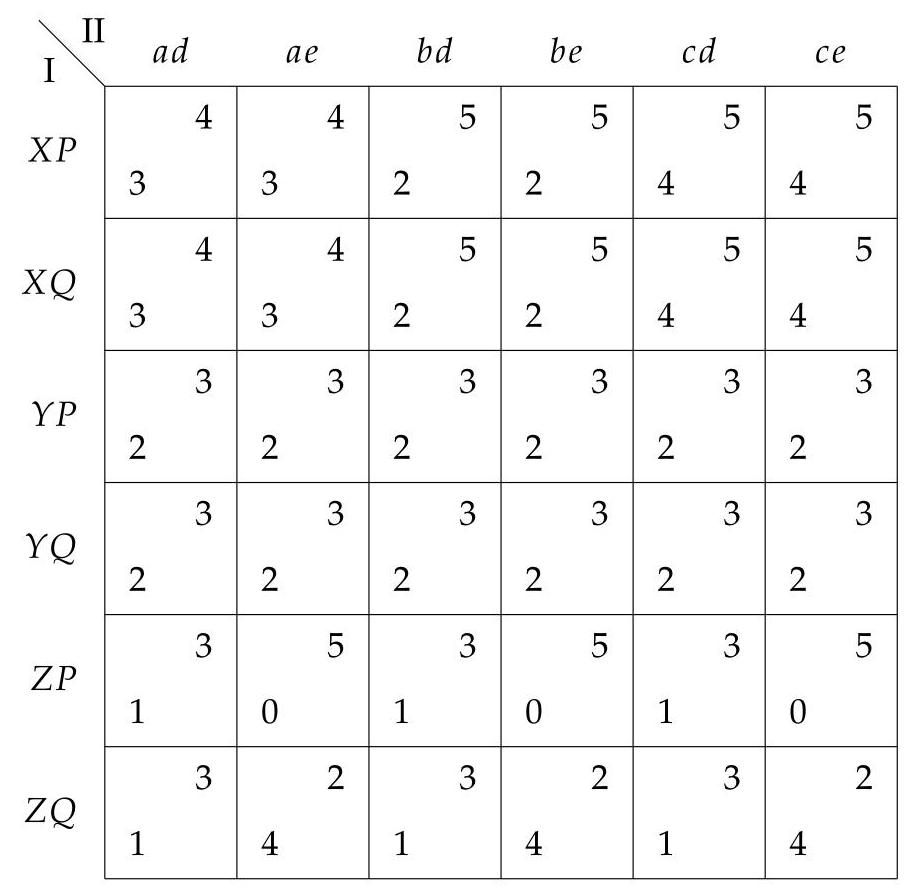
\includegraphics[width=0.6\linewidth]{translation/images/ch04-fig06.jpg}
    \caption{图\ref{fig:4.1}中扩展式博弈的策略形式。冗余较少的精简策略形式如图\ref{fig:4.7}所示。}
    \label{fig:4.6}
  \end{figure} 
 

以这种方式对无法到达的节点上的行动不做具体规定，根据以下定义确定了一个精简策略。由于由此产生的期望收益仍然是唯一确定的，将这些精简策略和由此产生的精简策略组合的收益制成表格，就得到了博弈的精简策略形式。图\ref{fig:4.1}中博弈树的精简策略形式如图\ref{fig:4.7}所示，并标明了最优反应收益。

\begin{definition}\label{def:4.5}
    在博弈树中，参与人的精简策略为该参与人的每个决策节点指定一个行动，但由于参与人自己先前的行动而无法到达的决策节点除外，在这些节点上，行动用“*”代替。精简策略组合是一个精简策略的元组，每个参与人对应一个。博弈树的精简策略形式列出了每个参与人的所有精简策略，并将每个精简策略组合下每个参与人的期望收益制成表格。
\end{definition}

  \begin{figure}[H]
    \centering
    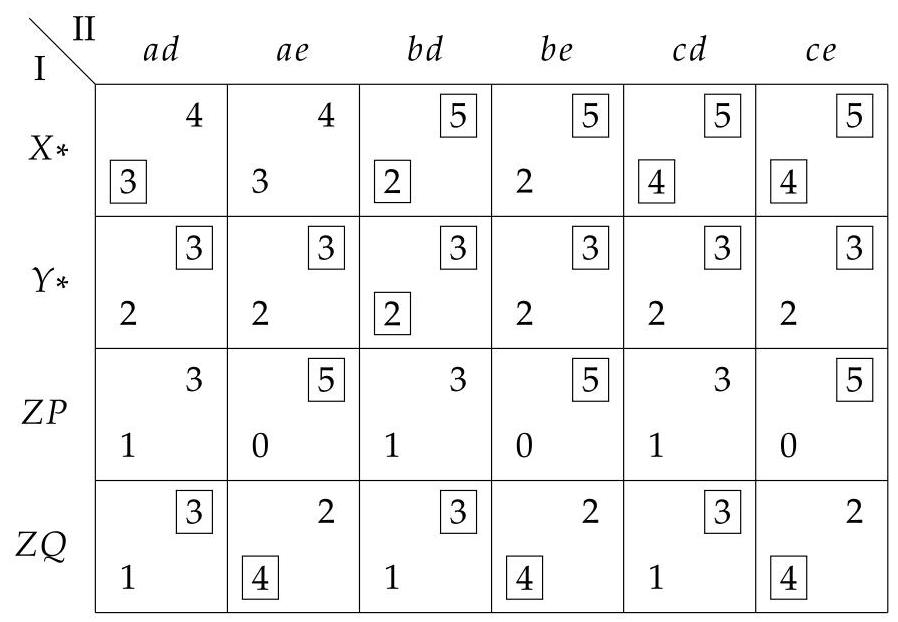
\includegraphics[width=0.8\linewidth]{translation/images/ch04-fig07.jpg}
    \caption{图\ref{fig:4.1}中扩展式博弈的精简策略形式。星号*代表参与人 I 在第二个决策节点上的任意行动，在行动 \(X\) 或 \(Y\) 之后无法到达该节点。}
    \label{fig:4.7}
  \end{figure}

上述定义对定义 4.3 和 4.4 进行了推广。重要的是，唯一未明确指定的行动是在由于参与人自身先前的行动而无法到达的决策节点处。一个精简策略不能因为另一个参与人可能不会在某个节点行动就忽略该行动，因为仅通过查看参与人自身的行动无法排除这种可能性。例如，在图\ref{fig:4.1}的博弈树中，参与人 II 的策略无法进行精简，因为她在一个决策节点的任何行动都不会排除她在另一个决策节点的行动。因此，在该博弈中参与人 II 的精简策略与她的(未精简的、原始的)策略相同。

在定义 4.5 中，精简策略的定义与收益无关，仅取决于博弈树的结构。可以通过识别对两个参与人都有相同收益的策略，并用一个单一的精简策略替换它们，从图\ref{fig:4.6} 的策略形式推导出图\ref{fig:4.7}的精简策略形式。一些作者根据策略形式中重复策略的消除来定义精简策略形式。(有时，在定义精简策略形式时也会消除(被占优) 策略。)我们在定义精简策略形式时不考虑收益，因为由于博弈叶节点的特殊收益，策略可能偶然具有相同的收益(这在通有博弈中不会发生)。此外，我们更倾向于让精简策略参考博弈树的结构，而不是收益的某种关系，这是博弈的不同方面。

以下是一个相对快速地填写类似图\ref{fig:4.1}这样的博弈树的精简策略形式(或者，如果愿意，完整策略形式)收益表的方法:

\begin{itemize}
\item 为每个参与人选择一个固定的决策节点顺序，树中较早出现的节点应排在前面。如果参与人有 \(k\) 个决策节点，一个(精简)策略有 \(k\) 个“空位”来定义一个行动，每个决策节点对应一个空位。
\item 生成所有(精简)策略。一个精简策略为每个空位定义一个行动，如果相应的决策节点由于同一参与人先前的行动而无法到达，则定义为未指定的行动“ \(*\) ”。对于两个参与人，将参与人 I 的(精简)策略列为行，参与人 II 的(精简)策略列为列。
\item 对于博弈树的每个叶节点，考虑从根节点到该叶节点的路径。首先假设该路径上没有机会行动。对于每个参与人，考虑该参与人在该路径上的行动。例如，图\ref{fig:4.1}中最左边的叶节点，收益为 $(3,4)$，参与人 I 的行动为 \(X\) ，参与人 II 的行动为 \(a\) 。
\item 对于每个参与人，识别所有与到达叶节点路径上的行动一致的策略。对于图\ref{fig:4.1}中最左边的叶节点和图\ref{fig:4.7}中的精简策略形式，这些策略对于参与人 \(\mathrm{I}\) 由精简策略 \(X *\) 给出(或者在图\ref{fig:4.6}中是未精简策略 \({XP}\) 和 \({XQ}\) )，对于参与人 II 是策略 \({ad}\) 和 \({ae}\) 。对于所有这些策略对，将收益对(这里是$(3,4)$)填入相应的单元格。对每个叶节点重复此操作。再举一个例子，直接跟随行动 \(Y\) 且收益为 $(2,3)$的叶节点，是由参与人 I 的行动 \(Y\) 到达的(该行动在图\ref{fig:4.7}的精简策略形式中定义了行 \(Y *\) )，参与人 II 没有行动，所以参与人 II 的所有策略都与这些行动一致；也就是说，整行 \(Y *\) 都填入收益对 $(2,3)$。
\item 如果从根节点到叶节点的路径上有机会行动，令 \(p\) 为该路径上机会概率的乘积。将叶节点的每个收益乘以 \(p\) ，并将结果加到如前所述确定的相应单元格的当前收益中(假设每个单元格的初始收益为零)。示例见图\ref{fig:4.8}。
\end{itemize}

这种创建博弈树策略形式的方法比考虑每对策略并确定它通向哪个叶节点(或者，如果有机会行动，则是哪些叶节点)要省力得多。

然而，应该清楚的是，策略形式通常比博弈树大得多。因此，直接分析博弈树通常比分析策略形式更容易。

策略是行动的组合，因此对于参与人的每个额外决策节点，该节点的每个行动都可以与已经考虑过的行动组合相结合。因此，行动组合的数量通常会随着参与人的决策节点数量呈指数增长。

  \begin{figure}[H]
    \centering
    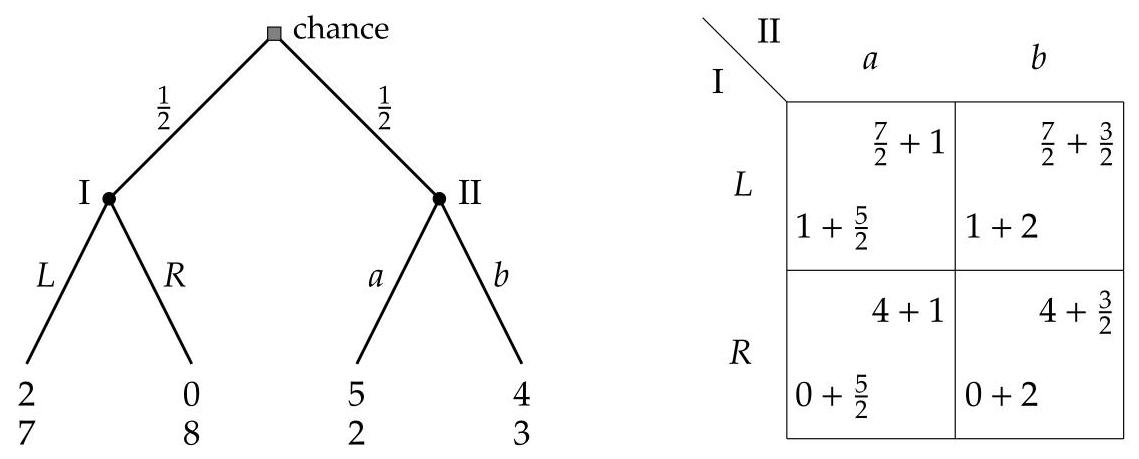
\includegraphics[width=0.8\linewidth]{translation/images/ch04-fig08.jpg}
    \caption{当存在导致期望收益的机会行动时，通过遍历博弈树的叶节点来创建策略形式。}
    \label{fig:4.8}
  \end{figure}

  \begin{figure}[H]
    \centering
    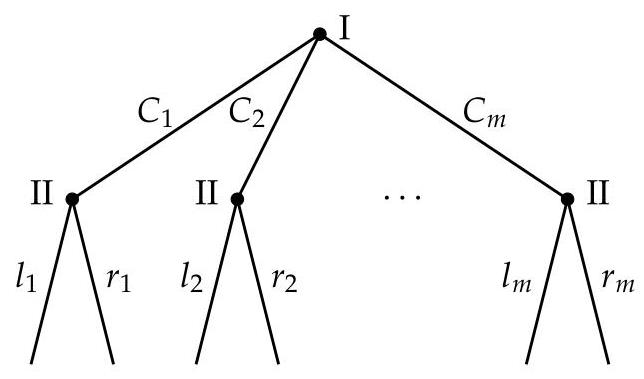
\includegraphics[width=0.6\linewidth]{translation/images/ch04-fig09.jpg}
    \caption{博弈树(无收益值)，参与人 I 在博弈树的根节点有 \(m\) 个行动 \({C}_{1},\ldots ,{C}_{m}\) 。在参与人 I 的每次行动 \({C}_{i}\) 之后，参与人 II 有两个行动 \({l}_{i}\) 和 \({r}_{i}\) 。参与人 II 有 \({2}^{m}\) 个策略。}
    \label{fig:4.9}
  \end{figure}

其原因在于，策略数量是各节点行动数量的乘积。例如，在图\ref{fig:4.9}的博弈中，参与人 I 有 \(m\) 种可能的初始行动，每次之后参与人 II 都有两种可能的行动，参与人 II 的策略数量是 \({2}^{m}\) 。此外，这也是参与人 II 的精简策略数量，因为无法进一步精简。这表明，即使是精简策略形式在博弈树的规模上也可能呈指数级增长。如果一个参与人的行动之前有自己的早期行动，那么精简策略形式会更小，因为在任何不选择前面自己行动的精简策略中，该行动可以不被确定。

\(\Rightarrow\) 练习~\ref{exer:4.4} 是关于精简策略的。

在精简策略形式中，如同定义 3.1 一样，均衡被定义为一个精简策略的组合，其中每个策略都是对其他策略的最优反应。在这种情况下，为了简洁起见，我们有时会简单地将精简策略称为“策略”。这是合理的，因为在考虑精简策略形式时，占优和均衡的概念可以直接应用于精简策略形式，例如应用于定义两人博弈的表格。那么“策略”就简单地意味着该表格中的一行或一列。“精简策略”这个术语仅在提及博弈树时才相关。

图\ref{fig:4.7}中的均衡被确定为那些(精简)策略对，它们彼此是最优反应，并且在表格的相应单元格中，两个收益值都被框起来。这些精简策略的均衡是 \(\left( {X*,{bd}}\right)\) 、 \(\left( {X*,{cd}}\right) ,\left( {X*,{ce}}\right)\) 和 \(\left( {Y*,{bd}}\right)\) 。

\section{子博弈精炼纳什均衡}\label{sec:4.6}

在本节中，我们考虑逆向归纳法和均衡之间的关系。均衡的概念基于策略形式，因为它适用于一个策略组合。在博弈树中，假设该组合中的策略是参与人在博弈开始前选择的，并且最优反应的概念假设其他参与人按照策略组合中的行动进行博弈。

以博弈树作为博弈的给定规范，通常希望保留其顺序解释。因此，参与人选择的策略也应该表达出逆向归纳法所表达的某种“顺序理性”。也就是说，策略组合中的行动对于博弈的任何部分都应该是最优的，包括由于早期行动(可能是其他参与人的行动)而无法到达的子树，就像图\ref{fig:4.3}(a)中威胁博弈中以参与人 II 的决策节点开始的小树一样。

在博弈树中，子博弈是博弈的任何子树，由树的一个节点作为子树的根节点及其所有后代节点给出。(注意:这个子博弈的定义仅适用于具有完美信息的博弈，这是我们目前考虑的博弈树。在第 10 章中我们将考虑的不完美信息扩展式博弈中，一个子树只有在所有参与人都知道他们处于该子树时才是一个子博弈；见第 10.10 节。)一个为每个子博弈定义均衡的策略组合被称为子博弈精炼纳什均衡或SPE。

\begin{theorem}\label{theo:4.6}
    逆向归纳法定义了一个子博弈精炼纳什均衡。
\end{theorem}

\begin{proof}
回顾逆向归纳法的过程：从最接近叶节点的节点开始，考虑一个决策节点 \(u\) ，假设 \(u\) 的所有后代节点的行动都已经被选择。在 \(u\) 的行动中，选择一个能使在 \(u\) 行动的参与人的期望收益最大化的行动。(如果在 \(u\) 之后有机会行动，则必须考虑期望收益。)以这种方式，为每个决策节点选择一个行动，从而确定一个完整的策略组合。

我们用归纳法证明该定理(见图\ref{fig:4.10}):考虑博弈树的一个非终端节点 \(u\) ，它可能是一个决策节点(如在逆向归纳法过程中)，也可能是一个机会节点。假设在节点 \(u\) 的行动为 \({c}_{1},{c}_{2},\ldots ,{c}_{k}\) ，这些行动会导向博弈树的子树 \({T}_{1},{T}_{2},\ldots ,{T}_{k}\) 。如果 \(u\) 是一个机会节点，那么我们有的不是行动，而是概率 \({p}_{1},{p}_{2},\ldots ,{p}_{k}\) 。作为归纳假设，假定到目前为止所选择的行动在每一棵子树中都定义了一个子博弈精炼纳什均衡（SPE）。(作为归纳的“基础情形”，对于每一棵只是树的叶节点的子树 \({T}_{1},{T}_{2},\ldots ,{T}_{k}\) ，这肯定是成立的；如果所有子树都是叶节点，那么 \(u\) 就是逆向归纳法过程中首先考虑的“最后”决策节点。)如果能证明通过在节点 \(u\) 选择行动，可以得到以 \(u\) 为根节点的子博弈的一个子博弈精炼纳什均衡，那么归纳步骤就完成了。

   \begin{figure}[H]
    \centering
    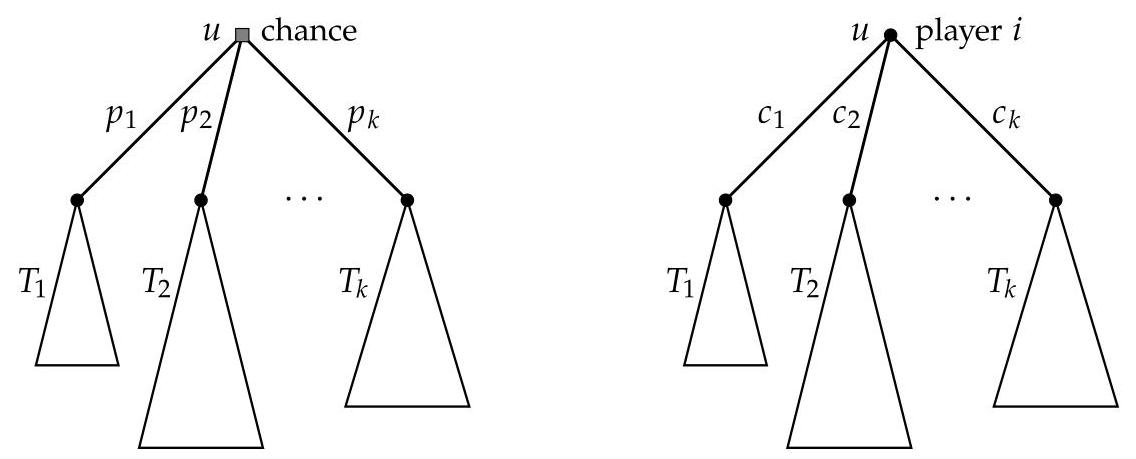
\includegraphics[width=0.8\linewidth]{translation/images/ch04-fig10.jpg}
    \caption{当下一个节点 \(u\) 属于机会(左图)或属于参与人 \(i\) (右图)时，证明定理~\ref{theo:4.6}的归纳步骤。}
    \label{fig:4.10}
  \end{figure}


首先，假设 \(u\) 是一个机会节点，这样下一个节点是根据博弈树中指定的固定概率来选择的。那么逆向归纳法不会为 \(u\) 选择行动，并且归纳步骤显然成立：对于每个参与人来说，从 \(u\) 开始的子博弈中的收益是子博弈 \({T}_{l}\) 的收益以概率 \({p}_{l}\) 对 \(1 \leq  l \leq  k\) 进行加权后的期望值，而且如果一个参与人能够提高该收益，她就必须通过改变至少一棵子树 \({T}_{l}\) 内的行动来实现，根据归纳假设，她无法做到这一点。

其次，假设 \(u\) 是一个决策节点，设 \(i\) 是在节点 \(u\) 行动的参与人，并考虑除参与人 \(i\) 之外的另一个参与人 \(j\) 。同样，对于参与人 \(j\) 来说，从 \(u\) 开始的子博弈中的行动是完全确定的。无论参与人 \(i\) 在节点 \(u\) 选择什么行动，参与人 \(j\) 都无法提高她的收益，因为这意味着她已经可以在某棵子树 \({T}_{l}\) 中提高她的收益了。

第三，考虑在节点 \(u\) 行动的参与人 \(i\) 。逆向归纳法会为节点 \(u\) 选择一个在其余行动给定的情况下对参与人 \(i\) 来说最优的行动。假设参与人 \(i\) 可以通过选择某个行动 \({c}_{l}\) 并额外改变他在子树 \({T}_{l}\) 中的行动来提高他的收益。但由此得到的提高后的收益仅仅是子树 \({T}_{l}\) 中提高后的收益，也就是说，该参与人本来就可以在子树 \({T}_{l}\) 中获得更好的收益。这与到目前为止所选择的行动为子树 \({T}_{l}\) 定义了一个子博弈精炼纳什均衡的归纳假设相矛盾。这样就完成了归纳。
\end{proof}

定理~\ref{theo:4.6}有两个重要的推论。在逆向归纳法中，每个行动都可以确定性地选择，因此逆向归纳法确定了一个纯策略组合。因此，定理~\ref{theo:4.6}意味着博弈树存在均衡，而且没有必要考虑随机策略。其次，子博弈精炼纳什均衡是存在的。对于博弈树，我们可以将“子博弈精炼纳什均衡（SPE）”与“通过逆向归纳法得到的策略组合”同义使用。

推论4.7:每个具有完美信息（perfect information）的博弈树都有一个纯策略均衡。

推论4.8:每个具有完美信息的博弈树都有一个子博弈精炼纳什均衡。

子博弈精炼纳什均衡（SPE）只能被描述为未精简(即完全明确)策略的组合。回顾图\ref{fig:4.1}中的博弈，子博弈精炼纳什均衡是 \(\left( {{XQ},{bd}}\right) ,\left( {{XQ},{cd}}\right)\) 和 \((YQ,bd)\)。图\ref{fig:4.7}中博弈的精简策略形式展示了均衡 \(\left( {X*,{bd}}\right) ,\left( {X*,{cd}}\right)\) 和 \(\left( {Y*,{bd}}\right)\) 。然而，我们不能将这些中的任何一个称为子博弈精炼纳什均衡，因为它们没有明确参与人 I 的第二步行动，如 \(*\) 符号所示。在这种情况下，在所有情况下将 \(*\) 替换为 \(Q\) 会得到一个子博弈精炼纳什均衡。要确定它们是否在每个子博弈中都定义了一个均衡，完整的策略是必要的。如图\ref{fig:4.7}所示，该博弈还有均衡 \(\left( {X*,{ce}}\right)\) 。这不是子博弈精炼的，因为它规定了行动 \(e\) ，而这不是以参与人 II 在 \(d\) 和 \(e\) 之间进行选择的决策节点开始的子博弈中的均衡的一部分:在该子博弈中，将 \(*\) 替换为 \(P\) 不是参与人 I 对 \(e\) 的最优反应，并且当将 \(*\) 替换为 \(Q\) 时，参与人 II 的最优反应不会是 \(e\) 。这一性质只能在博弈树中看到，即使在图\ref{fig:4.6}的未精简策略形式中也看不到，因为它涉及到由于参与人 \(\mathrm{I}\) 更早的行动 \(X\) 而未到达的博弈树部分。

\(\Rightarrow\) 练习~\ref{exer:4.3} 对于理解子博弈精炼纳什均衡非常有启发性。练习~\ref{exer:4.5} 研究了一个三人博弈。

\section{承诺博弈}

博弈树和策略型博弈之间的主要区别在于，在博弈树中，参与人按顺序行动，并且知道其他参与人之前的任何行动。相比之下，在策略型博弈中，参与人同时行动。当将一个两人的策略型博弈转变为承诺博弈时，这两种描述之间的差异变得非常明显。

承诺博弈是从一个两人的策略型博弈中得到的新博弈。其中一个参与人(我们总是选择参与人 I)先行动，选择他的一个策略。然后，与策略形式不同的是，参与人 II 会得知参与人 I 的行动，然后再行动。参与人 II 选择她原来的一个策略，这个策略可以取决于参与人 I 的行动。两个参与人最终获得的收益与原博弈中规定的相同。

图\ref{fig:4.11}展示了一个例子。(a)中的策略型博弈是图\ref{fig:3.2}(b)中的产品质量博弈。(b)和(c)中展示的承诺博弈是一个具有完美信息的博弈树，其中参与人 I 先行动，参与人 II 后行动。参与人 \(\mathrm{I}\) 原来的策略 \(T\) 和 \(B\) 变成了他的行动 \(T\) 和 \(B\) 。在图\ref{fig:4.11}(b)中，我们将参与人 II 随后的选择展示为两个 \(1 \times  2\) 博弈，它们是(b)中策略形式的两行，这取决于参与人 \(\mathrm{I}\) 的行动 \(T\) 或 \(B\) ，收益与(a)中相同。参与人 \(\mathrm{{II}}\) 然后可以分别在 \(l\) 和 \(r\) 之间进行选择。我们假设参与人 II 选择她的最优行动，由最优反应收益所示，即对 \(T\) 的反应是 \(l\) ，对 \(B\) 的反应是 \(r\) 。我们假设参与人 I 预期到了参与人 II 的这一行动，因此选择 \(T\) ，如逆向归纳箭头所示。
   \begin{figure}[H]
    \centering
    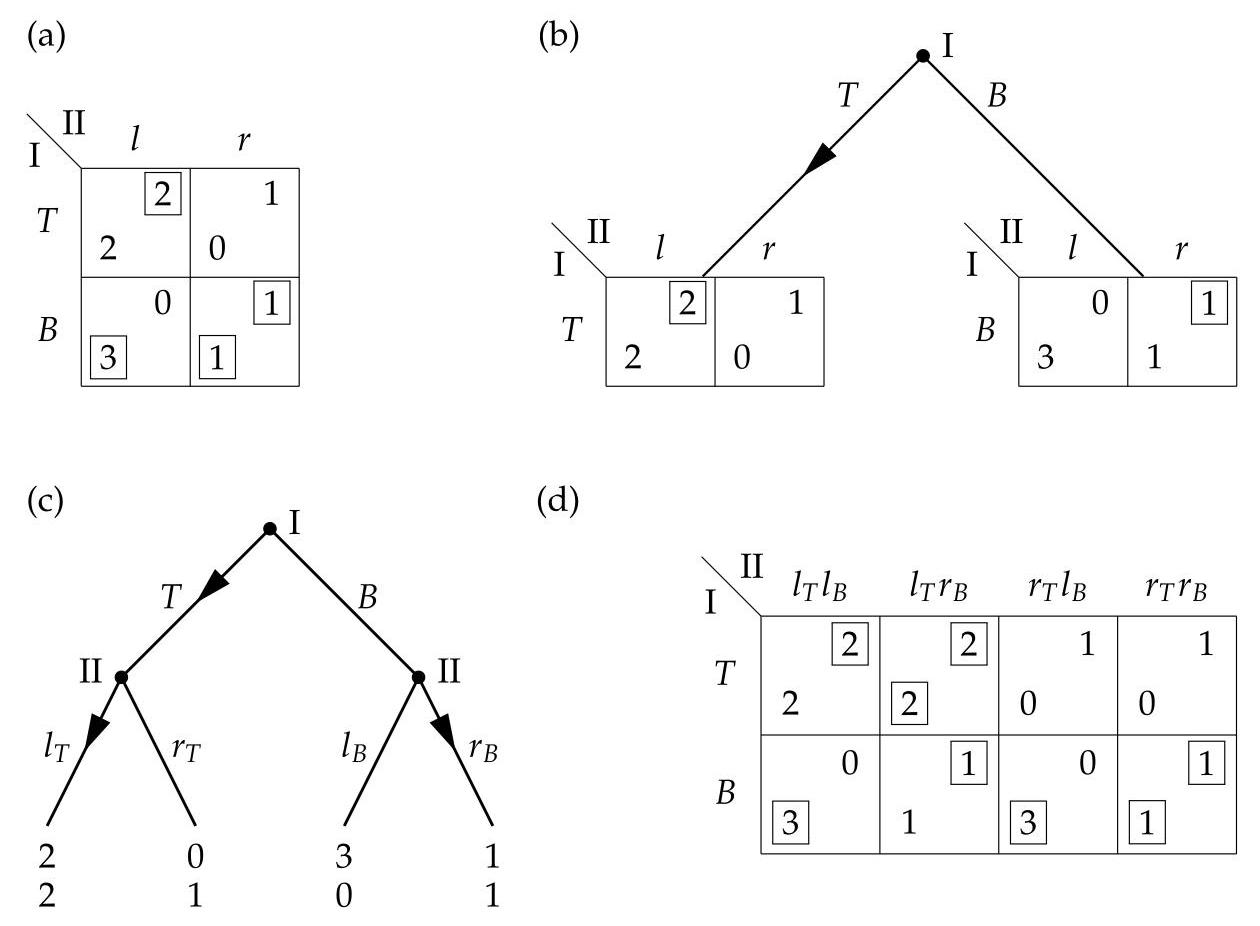
\includegraphics[width=0.8\linewidth]{translation/images/ch04-fig11.jpg}
    \caption{图\ref{fig:3.2}(b)中的同时进行的产品质量博弈(a)，转换为顺序的承诺博弈(b)，其中参与人 I 先行动，参与人 II 可以对参与人 I 的行动做出反应。(b)的传统表示形式是扩展式博弈(c)。(b)和(c)中的箭头显示了逆向归纳的结果。(c)带有最优反应收益的策略形式在(d)中展示。}
    \label{fig:4.11}
  \end{figure}


图\ref{fig:4.11}(b)中的图形描述仅说明了如何从原始的策略型博弈中得到承诺博弈。它表示一个博弈树，如图(c)所示，其中参与人 I 的每一步行动都会为参与人 II 产生一个单独的决策节点，参与人 II 的行动就是其原始策略。为了强调这些行动 \(l\) 和 \(r\) 是相互独立的，并且依赖于决策节点，我们在图(c)中给它们加上了下标，并将在行动 \(T\) 之后的行动称为 \({l}_{T}\) 和 \({r}_{T}\) ，在行动 \(B\) 之后的行动称为 \({l}_{B}\) 和 \({r}_{B}\) 。图\ref{fig:4.11}(d)展示了承诺博弈的策略形式。它表明原始的策略型博弈和承诺博弈有很大的不同。

在承诺博弈中，我们寻找子博弈精炼纳什均衡，也就是应用逆向归纳法。图\ref{fig:4.11}(b)和(c)表明，得到的唯一子博弈精炼纳什均衡是 \(\left( {T,{l}_{T}{r}_{B}}\right)\) ，这意味着(逆向推导)当参与人 II 面对高质量 \(T\) 时选择 \({l}_{T}\) ，面对低质量 \(B\) 时选择 \({r}_{B}\) 。因此，参与人 I 会选择 \(T\) ，因为这会给他带来更高的收益 2，而选择 \(B\) 只能得到 1。

与原始产品质量博弈中的均衡相比，承诺博弈(在子博弈精炼纳什均衡中)给两个参与人都带来了更高的收益。这是因为博弈发生了变化。重要的是，参与人 I 有能力承诺选择 \(T\) ，并且在看到参与人 II 选择 \(l\) 后不能再改回 \(B\) 。如果参与人 I 没有这种承诺能力，参与人的行为就不会如上述描述，博弈树也就不能准确反映该博弈。

图\ref{fig:4.11}中的承诺博弈还展示了均衡(一种策略组合)和均衡路径(当参与人使用其均衡策略时，博弈中实际采取的行动所描述的路径)之间的区别。(如果博弈没有机会行动，均衡路径就是博弈树中从根节点到叶节点的一条路径；如果博弈有机会行动，路径可能会分叉。)相比之下，一个策略组合定义了博弈树中每个部分的行动。这里，子博弈精炼纳什均衡 \(\left( {T,{l}_{T}{r}_{B}}\right)\) 为参与人 II 的两个决策节点指定了行动 \({l}_{T}\) 和 \({r}_{B}\) 。在均衡路径上，参与人 I 的行动是 \(T\) ，随后是参与人 II 的行动 \({l}_{T}\) 。然而，仅仅称这个均衡为 \(\left( {T,{l}_{T}}\right)\) 或 $(T,l)$是不够的，因为必须指定参与人 II 的行动 \({r}_{B}\) ，才能知道 \(T\) 是参与人 I 的最优反应。

我们在分析承诺博弈时只考虑子博弈精炼纳什均衡。例如，图\ref{fig:4.11}(a)中原始产品质量博弈的均衡 $(B,r)$也可以在图(d)中找到，其中参与人 II 总是选择与她在图(a)中的均衡策略相对应的行动 \(r\) ，这在承诺博弈中定义了策略 \({r}_{T}{r}_{B}\) 。这就确定了图(d)中的均衡 \(\left( {B,{r}_{T}{r}_{B}}\right)\) ，因为 \(B\) 是对 \({r}_{T}{r}_{B}\) 的最优反应，而 \({r}_{T}{r}_{B}\) 是对 \(B\) 的最优反应。然而，这个承诺博弈的均衡不是子博弈精炼的，因为它规定了在均衡路径之外采取次优行动 \({r}_{T}\) ；这并不影响均衡性质，因为参与人 I 不会选择 \(T\) 。(这是一个一般论证：考虑原始博弈的任何均衡$(x,y)$，在承诺博弈中让参与人 I 承诺选择 \(x\) ，让参与人 II 总是以 \(y\) 回应；那么这就是承诺博弈的一个均衡，但一般来说它不是子博弈精炼的。)

为了以一种有趣的方式比较策略型博弈和其承诺博弈，我们只考虑承诺博弈的子博弈精炼纳什均衡。

在实际应用中，人们通常关心“改变博弈规则”之后会发生什么，并用适当的博弈论分析来考察其结果。将产品质量博弈转变为承诺博弈，能展示出双方参与人如何从中受益。

承诺博弈也被称为领导博弈，在这种博弈中，先行动的参与人被称为领导，后行动的参与人被称为跟随者。领导不可撤销地坚持其策略的能力非常重要，这也被称为承诺能力。承诺能力通常会带来先行优势，即领导的处境不会比参与人同时行动的原始博弈更差(如练习~\ref{exer:4.7} 所示，当最优反应总是唯一时，这一点肯定成立)。

必须谨慎理解这一说法。例如，如果任何一方参与人都有承诺的能力，那么先行行动并不一定是最优选择。例如，考虑改变图\ref{fig:4.11}(a)中的博弈，让参与人 II 能够承诺其策略，而参与人 I 后行动。那么参与人 I 总是会选择 \(B\) 作为回应，因为这是他在(a)中的占优策略。然后，通过逆向归纳法，参与人 II 会选择 \(r\) ，参与人 I 会选择 \({B}_{l}{B}_{r}\) ，双方都只得到较低的收益 1。此时，正如先行优势所断言的，参与人 II 的处境并不比同时选择的博弈更差，但也没有获得任何好处。相比之下，如图\ref{fig:4.11}(b)所示，让参与人 I 先行动对双方都有利。

承诺博弈也被称为斯塔克尔伯格博弈，这是以经济学家海因里希·冯·斯塔克尔伯格(Heinrich von Stackelberg)的名字命名的，他将这种博弈应用于古诺双寡头产量竞争，比如我们在第 3.6 节中考虑的博弈。我们首先研究图\ref{fig:3.8}中该承诺博弈的有限版本，然后研究任意非负 \(x\) 和 \(y\) 情况下的无限版本(3.6)。我们会发现，在这个博弈中，领导的处境比同时行动的博弈更好，但跟随者的处境更差。

图\ref{fig:3.8}中博弈的承诺博弈如图\ref{fig:4.12}所示，就像图\ref{fig:4.11}(b)是从图\ref{fig:4.11}(a)推导出来的一样。参与人 II 的最优反应由她对参与人 I 的第一步行动 0、3、4、6 的(原博弈中的)最优反应给出，分别为 6、4、4、3，对应的收益对分别为 \(\left( {0,{36}}\right) ,\left( {{15},{20}}\right) ,\left( {{16},{16}}\right)\) 和 \(\left( {{18},9}\right)\)。其中，18 是参与人 I 能得到的最高收益。因此，通过逆向归纳法，参与人 I 会承诺选择最右边的行动 6。相应的收益是参与人 I 为 18，参与人 II 为 9，而在图\ref{fig:3.8}的同时行动博弈中，双方的收益均为 16。在这个对称博弈中，一方参与人可信地承诺自己策略的能力为领导带来了明显的先行优势，与产品质量博弈不同的是，这里是以牺牲跟随者的利益为代价的。

现在我们考虑在(3.6)中，当参与人 I 和参与人 II 的策略 \(x\) 和 \(y\) 是 \(\left\lbrack  {0,{12}}\right\rbrack\) 中的任意实数时(他们不会选择 \(x > {12}\) 或 \(y > {12}\) ，因为这会给他们带来负收益)，该博弈的承诺博弈。我们已经知道，参与人 II 对 \(x\) 的最优反应是 \(y\left( x\right)  = 6 - x/2\) 。在承诺博弈中，将参与人 II 的选择看作是参与人 \(\mathrm{I}\) 的承诺 \(x\) 的函数 \(y\left( x\right)\) 确实很有用。

   \begin{figure}[H]
    \centering
    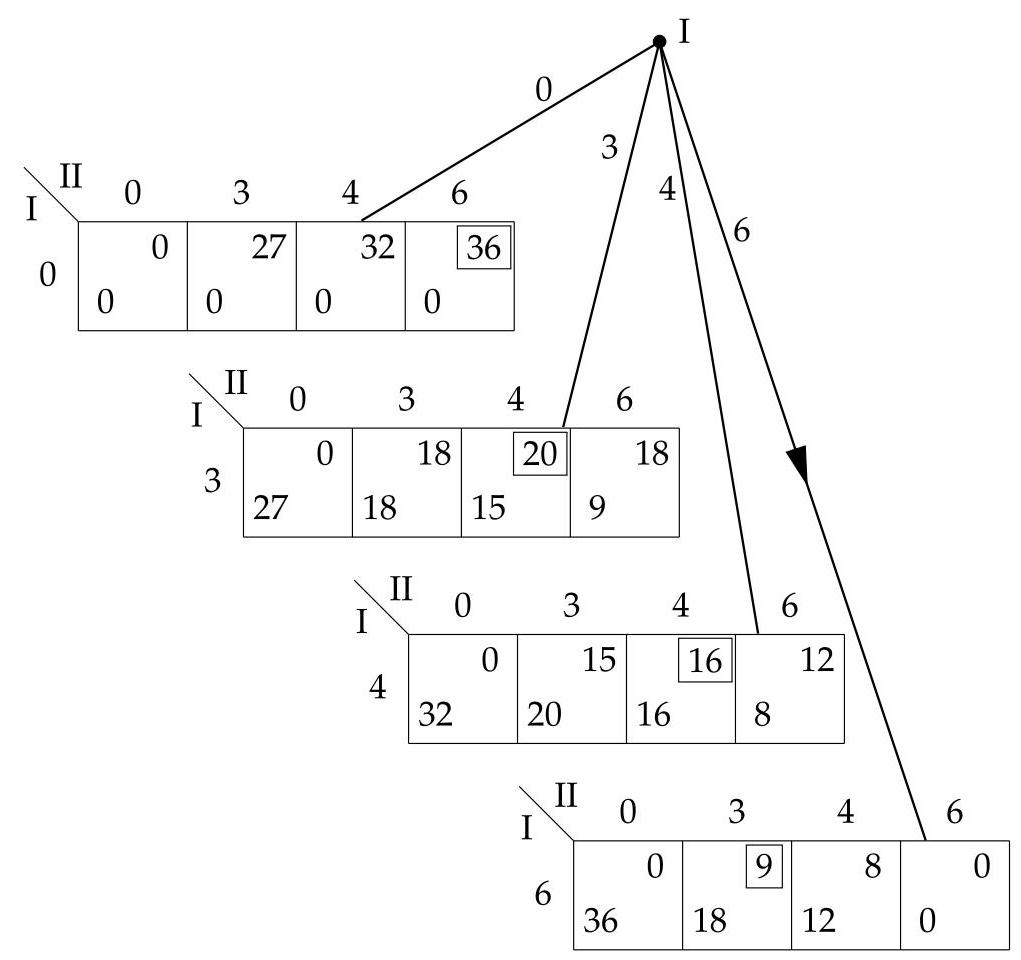
\includegraphics[width=0.8\linewidth]{translation/images/ch04-fig12.jpg}
    \caption{图\ref{fig:3.8}中双寡头博弈的承诺博弈。}
    \label{fig:4.12}
  \end{figure}


与承诺博弈中一贯的做法一样，我们寻找子博弈精炼纳什均衡（SPE），并假设跟随者即使在非均衡路径上也会选择其最优反应。因此，逆向归纳法的结果是选择 \(x\) 来最大化 \(a\left( {x,y\left( x\right) }\right)\)，即最大化 \(x\cdot(12-y(x)-x)=x\cdot(6-x/2)=6x-x^2/2\)。该函数关于 \(x\) 的导数为 \(6 - x\) ，当 \(x = 6\) 时为零。也就是说，参与人 I 承诺选择 6，而参与人 II 对于任何承诺 \(x\) 都会以 \(y\left( x\right)  = 6 - x/2\) 作为回应(这定义了参与人 II 在这个子博弈精炼纳什均衡中的完整策略)，特别是在均衡路径上以 \(y\left( 6\right)  = 3\) 回应。最终结果是参与人 I 的收益为 18，参与人 II 的收益为 9。策略 6 和 3 是图\ref{fig:3.8} 中 \(4 \times  4\) 博弈的一部分，同时还有该同时博弈中两个参与人的均衡策略 4。

\(\Rightarrow\) 练习~\ref{exer:4.7} 研究了一个像\eqref{eq:3.6} 那样具有无限策略集的博弈，并做出了有趣的观察，特别是在(d)中，比较了承诺博弈与原始同时博弈中两个参与人的收益。

\section{延伸阅读}

逆向归纳法也被称为策梅洛算法，这一名称源于策梅洛(1913 年)关于国际象棋的一篇文章。然而，策梅洛关注的并非逆向归纳法，而是证明了如果白方能够迫使获胜，那么他可以在有限步数内做到这一点(施瓦尔贝和沃克，2001 年)。因此，“逆向归纳法”是更合适的术语。

精简策略有时是根据策略形式来定义的，即通过识别对所有参与人具有相同收益的策略。我们仅通过博弈树的结构独立于收益来定义这种精简，这样更清晰。我们还为每个未指定的行动和每个决策节点(可能有多个这样的决策节点)给出 * 符号(有时会省略)，以确保即使是精简策略，当参与人有 \(k\) 个决策节点时也有 \(k\) 个“行动槽”。

经济学家冯·斯塔克尔伯格(1934 年)分析了企业在双头垄断情况下的各种行为方式，其中之一就是领导博弈，即一家企业承诺一定的产量，而另一家企业以最优反应做出回应。我们用现代博弈论的概念描述了这一情况(另见吉本斯，1992 年)，这些概念在 1934 年还不存在。

在第 4.7 节末尾讨论的博弈\eqref{eq:3.6} 的承诺博弈是一个对称博弈，参与人从一个区间中选择他们的策略，该博弈有唯一的对称均衡，并且参与人的最优反应函数是唯一的，并且随着另一个参与人的选择单调变化。由于该博弈是对称的，在相应的承诺博弈中，当参与人 \(\mathrm{I}\) 是领导时，分析该博弈就足够了，该博弈为领导和跟随者都带来了子博弈精炼纳什均衡收益。领导的收益至少与同时博弈中的收益一样高(见练习~\ref{exer:4.6})。奇怪的是，在这类博弈中，跟随者的收益要么比同时博弈中的收益差，要么甚至比领导的收益还高(如练习~\ref{exer:4.7})。也就是说，与同时博弈相比，两个参与人都从序贯博弈中获利，但领导比跟随者获利更多这种看似自然的情况并不会出现。证明过程很简短，只使用了一些单调性条件(冯·施滕格尔，2010 年，定理 1)。

\section{第 4 章练习}

\begin{exercise}\label{exer:4.1}
考虑以下博弈树。和往常一样，叶节点处的上方收益是参与人 I 的，下方收益是参与人 II 的。

(a) 参与人 I 和参与人 II 的策略数量分别是多少？
   \begin{figure}[H]
    \centering
    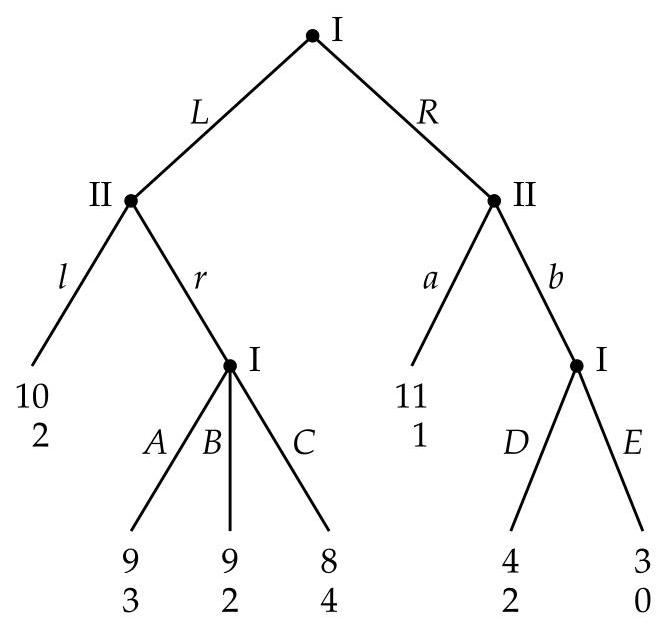
\includegraphics[width=0.6\linewidth]{translation/images/ch04-fig13.jpg}
    \caption{}
  \end{figure}

(b) 他们各有多少个精简策略？

(c) 给出该博弈的精简策略形式。

(d) 该博弈在精简策略下的均衡是什么？

(e) 该博弈的子博弈精炼纳什均衡是什么？
\end{exercise}

\begin{exercise}\label{exer:4.2}
考虑以下博弈树。

(a) 参与人 I 和参与人 II 的策略数量分别是多少？每个参与人各有多少个精简策略？
   \begin{figure}[H]
    \centering
    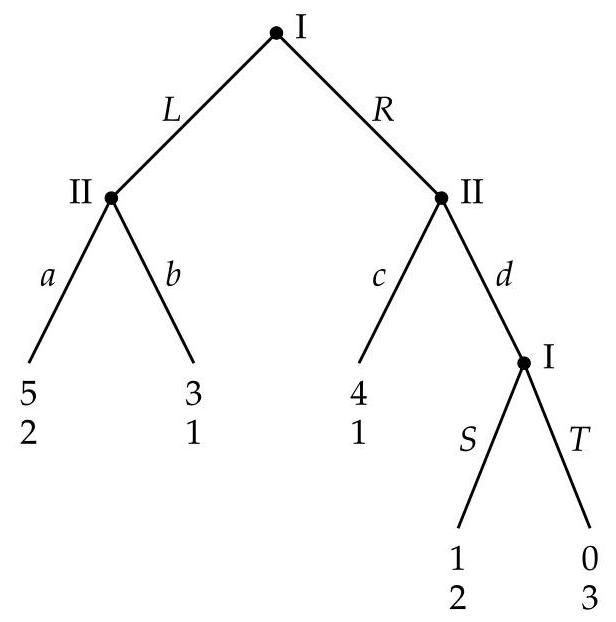
\includegraphics[width=0.6\linewidth]{translation/images/ch04-fig14.jpg}
    \caption{}
  \end{figure}


(b) 给出该博弈的精简策略形式。

(c) 该博弈在精简策略下的均衡是什么？该博弈的子博弈精炼纳什均衡是什么？

(d) 找出每一对精简策略，其中一个策略弱占优或严格占优于另一个策略，并指出这种占优是弱占优还是严格占优。
\end{exercise}

\begin{exercise}\label{exer:4.3}
考虑以下博弈树。
   \begin{figure}[H]
    \centering
    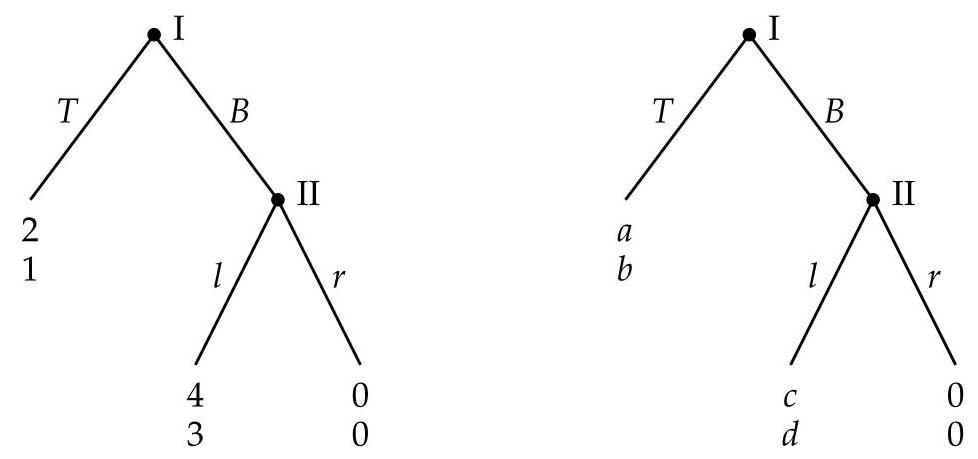
\includegraphics[width=0.8\linewidth]{translation/images/ch04-fig15.jpg}
    \caption{}
  \end{figure}


(a) 找出左边博弈树的所有均衡。其中哪些是子博弈精炼纳什均衡？

(b) 在右边的博弈树中，收益 \(a,b,c,d\) 是正实数。对于以下陈述 (i)、(ii)、(iii) 中的每一个，判断其是真还是假，并用论据或反例证明你的答案；你可以引用任何标准结果。对于任何 \(a,b,c,d > 0\) ，

(i) 该博弈始终存在子博弈精炼纳什均衡（SPE）；

(ii) 在任何子博弈精炼纳什均衡中，参与人 II 的收益总是至少不低于她在任何均衡中的收益；

(iii) 在任何子博弈精炼纳什均衡中，参与人 I 的收益总是至少不低于他在任何均衡中的收益。
\end{exercise}

\begin{exercise}\label{exer:4.4}
考虑以下两个博弈树 (a) 和 (b)。由于收益与问题无关，因此省略。在每种情况下，每个参与人有多少种策略？有多少种精简策略？

(a)
   \begin{figure}[H]
    \centering
    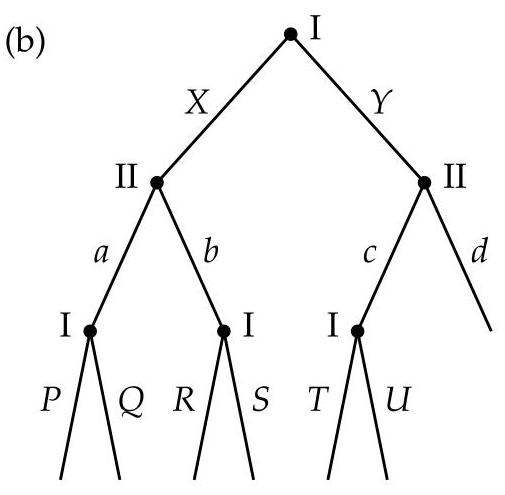
\includegraphics[width=0.4\linewidth]{translation/images/ch04-fig16.jpg}
    \caption{}
  \end{figure}
  
   \begin{figure}[H]
    \centering
    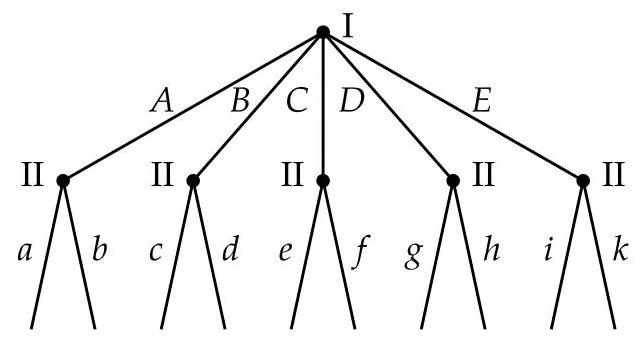
\includegraphics[width=0.4\linewidth]{translation/images/ch04-fig17.jpg}
    \caption{}
  \end{figure}


\end{exercise}

\begin{exercise}\label{exer:4.5}
考虑以下三人博弈树。在叶节点处，最上面的收益属于参与人 I，中间的收益属于参与人 II，最下面的收益属于参与人 III。


   \begin{figure}[H]
    \centering
    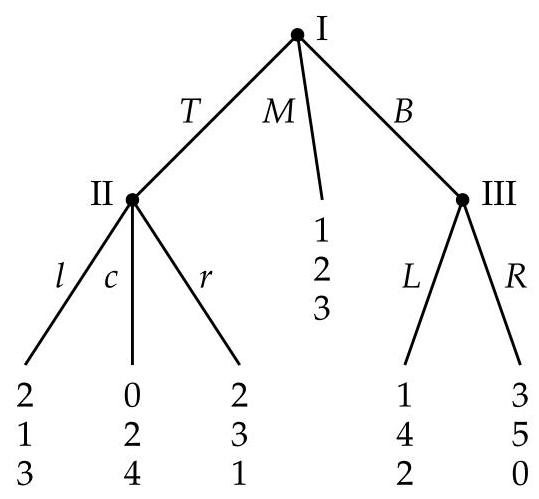
\includegraphics[width=0.4\linewidth]{translation/images/ch04-fig18.jpg}
    \caption{}
  \end{figure}
 
(a) 这个博弈有多少个策略组合？

(b) 找出所有一个策略严格或弱占优另一个策略的策略对。

(c) 找出所有(纯策略)均衡。其中哪些是子博弈精炼纳什均衡？
\end{exercise}

\begin{exercise}\label{exer:4.6}
考虑一个策略型博弈 \(G\) 。回顾一下，从 \(G\) 导出的承诺博弈的定义是，让参与人 I 选择他的一个策略 \(x\) ，然后将其告知参与人 II，参与人 II 随后可以在每种情况下选择 \(G\) 中的一个策略作为对 \(x\) 的回应。由此产生的收益与原始博弈 \(G\) 中的收益相同。

(a) 如果 \(G\) 是一个 \(m \times  n\) 博弈，在承诺博弈中，参与人 \(\mathrm{I}\) 和参与人 \(\mathrm{{II}}\) 分别有多少种策略？

对于以下每个陈述，判断它们是真还是假；通过简短的论证或反例来证明你的答案。

(b) 在承诺博弈的子博弈精炼纳什均衡中，参与人 I 永远不会选择一个在 \(G\) 中严格被占优的策略。

(c) 在承诺博弈的子博弈精炼纳什均衡中，参与人 II 永远不会选择一个在 \(G\) 中严格被占优的策略。
\end{exercise}

\begin{exercise}\label{exer:4.7}
设 \(G\) 为以下博弈：参与人 I 选择一个非负实数 \(x\) ，同时参与人 II 选择一个非负实数 \(y\) 。由此产生的(对称)收益为

\[
x \cdot  \left( {4 + y - x}\right) \;\text{，给参与人 }\mathrm{I}\text{，}
\]

\[
y \cdot  \left( {4 + x - y}\right) \;\text{，给参与人 II。}
\]

(a) 给定 \(x\) ，确定参与人 II 的最优反应 \(y\left( x\right)\) (它是 \(x\) 的函数)，以及参与人 I 对 \(y\) 的最优反应 \(x\left( y\right)\) 。找出一个均衡，并给出两个参与人的收益。

(b) 找出承诺博弈(参与人 I 先行动)的一个子博弈精炼纳什均衡，并给出两个参与人的收益。

(c) (a)和(b)中的均衡是否唯一？

(d) 设 \(G\) 为一个博弈，其中参与人 II 对参与人 I 的任何策略 \(x\) 的最优反应 \(y\left( x\right)\) 总是唯一的。证明在承诺博弈(参与人 I 先行动)的任何子博弈精炼纳什均衡（SPE）中，参与人 I 的收益至少不低于原博弈 \(G\) 中任何均衡下他的收益。
\end{exercise}
